\section*{\sffamily \Large ROBUST PCA WITH INDEPENDENT SAMPLES}
\label{Section:sec2}

\subsection*{\sffamily \large Robust covariance matrices, projection pursuit}

The early and by now well-established approaches to robust PCA were based on robustly estimating the population covariance matrix, and using eigenvectors of that estimate as principal components. Some methods of robust covariance matrix estimation include a projection-based estimator by \cite{maronna76}, the Minimum Volume Ellipsoid estimator \citep{Rousseeuw84},  the Minimum Covariance Determinant (MCD) estimator \citep{rousseeuw85} and the Stael-Donoho estimators \citep{MaronnaYohai95,ZuoCui05}. Although these methods have high breakdown points, they are not entirely suitable for many modern applications where one or more of $n$ and $p$ can be large, and $n < p$ is not uncommon. They typically require computation of the entire covariance matrix, which is not possible when $n < p$. Even when $n > p$, these methods become computationally intensive with large data dimensions.

\cite{LiChen85} introduced the idea of Projection Pursuit (PP) in robust PCA to alleviate these problems. They proposed to replace the variances in (\ref{eqn:eqnPCA1}) and (\ref{eqn:eqnPCAk}) by a robust univariate scale estimator $s_n$ (e.g. median, MCD), and obtain the robust PCs subsequently:
%
\begin{align*}
\hat \bfw_1^\text{PP} &= \argmax_{\| \bfw \| = 1} s_n ( \bfw^T \bfx_1, \ldots, \bfw^T \bfx_n );\\
\hat \bfw_k^\text{PP} &= \argmax_{\| \bfw \| = 1; \bfw \perp \bfw_s, s < k} s_n ( \bfw^T \bfx_1, \ldots, \bfw^T \bfx_n ) \quad \text{for } 1< k \leq p
\end{align*}
%
Aside from not having any restrictions for high-dimensional data, the PP approach allowed the flexibility of using any robust univariate scale estimator, and sequential estimation of the principal components. PP-based robust PCA became a popular method for chemometric data analysis in the 1990-s and early 2000-s, mainly due to the algorithmic developments by \cite{XieEtal93}, \cite{HubertEtal02} and \cite{CrouxEtal07}.

The ROBPCA method of \cite{hubert05} combines the above two approaches. Specifically, ROBPCA consists of the following steps:
%
\begin{enumerate}
\item Do an initial dimension reduction of the data matrix: $\bfX_{n \times p} \mapsto \bfZ_{n \times r}, r \leq p$ by projecting all data points on the subspace formed by the right singular vectors of $\bfX$:
%
$$
\bfX = \bfU_{n \times r} \bfD_{r \times r} \bfV_{r \times p}; \quad
\bfZ = \bfU \bfD
$$

\item Calculate the outlyingness of all samples:
%
$$
O(\bfz_i) = \max_{\bfv \in B} \frac{| \bfz_i^T \bfv - m_n (\bfz_j^T \bfv)|}{s_n (\bfz_j^T \bfv )}
$$
%
where $m_n$ and $s_n$ are robust location and scale estimators, respectively. The set of vectors $B$ is taken as the vectors passing through all possible pairs of sample points if $\binom{n}{2} < 250$, and a collection of 250 randomly chosen non-zero vectors in $\BR^{r}$ otherwise.

Use the top $k$ PCs calculated from the $h$ least outlying points ($k \leq r; k, h$ suitably chosen) to transform the data again:
%
$$
\bfZ^* =  \bfZ \bfP_0; \quad \bfP_0 \in \BR_{r \times k}
$$

%\item If $s_n (\bfz_j^T \bfv ) = 0$ for some $\bfv$, then all samples are projected onto the hyperplane orthogonal to that $\bfv$ and these projection are taken as the new observations to work with. This optional step potentially reduces data dimension to some $r_1 \leq r_0$. for notational convenience, we still refer to this transformed data as $\bfZ$.

\item Robustly estimate the scatter matrix of $\bfZ^*$, take its eigenvectors as the estimated robust PCs.
\end{enumerate}

As \cite{hubert05} showed through application on simulated and real data, the combination of a PP approach (first step) and robust scatter matrix estimation (third step) used by ROBPCA results in efficiency gains in estimating population principal components, as well as better detection of outlying points, compared to classical PCA, one of their previously proposed methods \citep{HubertEtal02}, as well as spherical and ellipsoidal PCA \citep{LocantoreEtal99}.

\subsection*{\sffamily \large Data transformation and M-estimation}

A parallel approach towards robust PCA has also been developed by researchers, that is focused on the usage of robust transformations on the data, specifically multivariate signs and ranks, and related $M$-estimates of scatter. Introduced by \cite{MottonenOja95}, the multivariate sign or \textit{spatial sign} of a vector $\bfx \in \BR^p$ with respect to a location parameter $\bfmu \in \BR^p$ is defined as:
%
$$
\bfS (\bfx) = \frac{\bfx  - \bfmu }{\| \bfx - \bfmu\|} \BI \{ \bfx \neq \bfmu \}
$$
%
where $\BI(.)$ is the 0/1 indicator function. When $\bfx$ is a random sample from an elliptical distribution, the sign transformation keeps the population eigenvectors constant. Since all vectors in the same direction get mapped to the same spatial sign regardless of their magnitude, eigenvector estimates calculated from the Sign Covariance Matrix (SCM), or equivalently the SVD of a sign transformed data matrix can act as robust PCs \citep{LocantoreEtal99,visuri00}.

\begin{figure}[t]
\centering
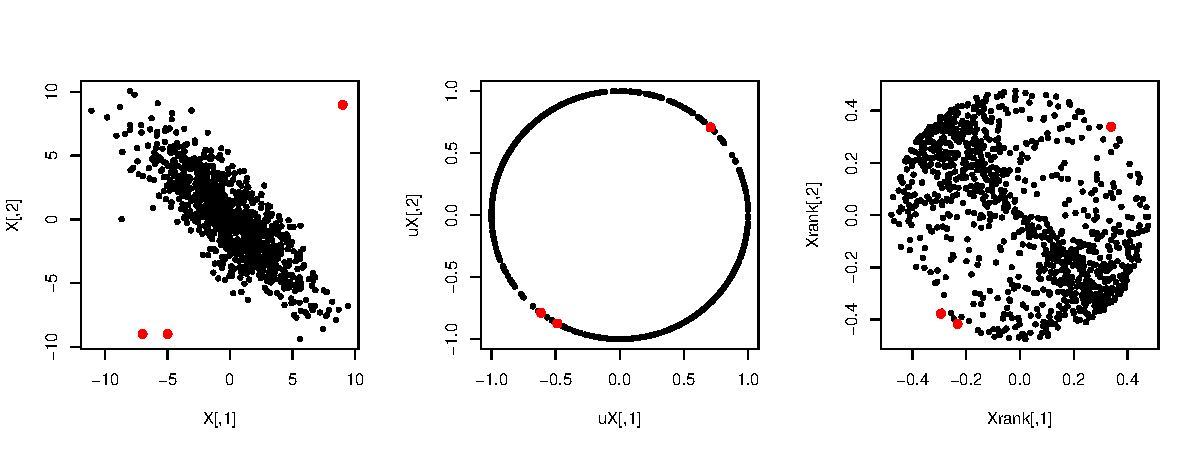
\includegraphics[width=\textwidth]{allthree}
	\caption{(Left) 1000 points randomly drawn from $\mathcal N_2\left((0,0)^T, \left(\protect\begin{smallmatrix} 5 & -4 \\ -4 & 5 \protect\end{smallmatrix}\right)\right) $ (in black), and three outliers (in red);\\
(Center) their spatial signs: all points reside on the surface of a finite ball in $\BR^2$;\\
(Right) their multivariate ranks based on halfspace depth: retains the shape of the data.}
	\label{fig1:allthree}
\end{figure}

There are two components of a multivariate data point: its direction and magnitude. Spatial sign discards the magnitude and only uses the direction. Consequently, although the sign transformation provides an intuitively simple way of robustly estimating population eigenvectors, the estimates are not very accurate in terms of asymptotic and finite-sample efficiencies \citep{Majumdar15}. In fact, \cite{magyar14} showed that the eigenvectors of the M-estimate of scatter proposed by \cite{tyler87} have uniformly lower asymptotic risk than those obtained from the SCM.

\cite{Majumdar15} rectified this by weighting the spatial signs by a bounded distance measure from the origin. They used data depth \citep{zuo00} to construct these weight functions. For some $\bfy \in \BR^p$ and a set of points in $\BR^p$, say $(\bfy_1, \ldots, \bfy_n)^T = \bfY$, data depth (denoted by $D(\bfy, \bfY)$) provides an affine invariant scalar measure of how close $\bfy$ is to the data cloud. The depth-based weighted spatial signs \citep{Majumdar15} are explicitly constructed as:
%
\begin{align}
\tilde \bfx = \left[ \sup_{\bfz} D(\bfz, \bfX) - D(\bfx, \bfX) \right] \bfS( \bfx - \bar \bfX )
\end{align}
%
The transformation $\bfx \mapsto \tilde \bfx$ preserves the magnitude information of a point: points with the same direction but different magnitudes get mapped further from the origin as the magnitude increases. However, due to the boundedness of data depth, this mapping limits the maximum distance an outlying point can get mapped to (see figure \ref{fig1:allthree}). Consequently, the weighted sign transformation improves upon the sign-based PCA in terms of lower estimation errors for elliptic underlying distributions, while still preserving robustness properties like high breakdown points and bounded influence functions \citep{Majumdar15}.

\subsection*{\sffamily \large Robust PCA and outlier detection}
Aside from obtaining a lower dimensional projection of the data matrix $\bfX$ in spite of outliers that is close enough to the projection of $\bfX$ by the first few population eigenvectors, detecting the outliers themselves is also closely associated with robust PCA. These samples can be of interest for mechanistic reasons. For example in the analysis of near infra-red absorbance for 39 gasoline samples over 226 wavelengths using ROBPCA (see \cite{hubert05}), six compounds are flagged as outliers, and these turn out to be the only samples containing alcohol. Over the past two decades, multiple approaches of using robust principal components for detecting anomalous samples have been proposed \citep{ShyuEtal03,JacksonChen04,BrownEtal10,PascoalEtal10}. In their 2005 paper, aside from the popular ROBPCA method \cite{hubert05} also introduced a notion of outlier diagnostics that is applicable to any method of robust PCA and can serve as a means to compare different relevant techniques as well.

\begin{figure}[t]
\centering
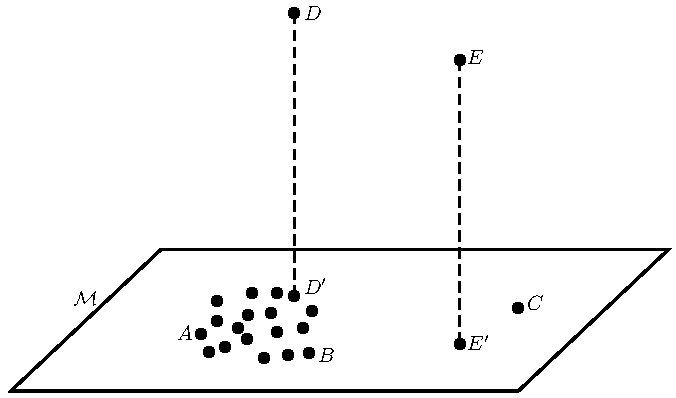
\includegraphics[width=.6\textwidth]{ROBPCA}
	\caption{Four different types of points in 3-dimensional data with respect to a 2-PC subspace: $A$ and $B$ are regular observations, $C$ is a good leverage point, $D$ is an orthogonal outlier, and $E$ is a bad leverage point.}
	\label{fig:figROBPCA}
\end{figure}

We illustrate this in Figure~\ref{fig:figROBPCA}. Here we consider data in 3 dimensions, and consider the relative position of samples with respect to the two-dimensional principal component subspace $\cM$. We can classify such points into four categories:

\begin{enumerate}
\item{\it Regular observations}: points that form a homogeneous group close to $\cM$ ($A$ and $B$ in figure);
\item{\it Good leverage points}: points that lie close to $\cM$, but at a distance from the regular observations ($C$ in figure);
\item{\it Orthogonal outliers}: These points (point $D$ in figure) lie far away from their projections on $\cM$ (point $D'$, but the projections themselves are close to the regular observations;
\item{\it Bad leverage points}: These points are also far away from their projections on $\cM$ ($E$ and $E'$ respectively), but the projections are also far away from the regular observations.
\end{enumerate}

\cite{hubert05} introduced the concept of \textit{score distance} (SD) and \textit{orthogonal distance} (OD) to distinguish between these four categories. With our notation, for the $i^\text{th}$ observation these distances are defined as:
%
$$
SD_i = \sum_{j=1}^q \frac{t_{ij}}{\lambda_j};\
\quad OD_i  =\| ( \bfI - \bfW_k \bfW_k^T) (\bfx_i - \bfmu) \|
$$
%
The SD can be interpreted as the weighted distance of the projection of a point on the hyperplane formed by the first $k$ PCs, while OD is the orthogonal distance of that point and the $k$-PC hyperplane. It is now clear from our picture that regular observations have low values of both SD and OD, while bad leverage points have high values of both. An orthogonal outlier has small SD but large OD, whereas a good leverage point has high SD but small OD. To explicitly classify sample points into these 4 categories, \cite{hubert05} use $\sqrt {\chi^2_{k,0.975}}$ and $[ \hat \mu (OD^{2/3}) + \hat \sigma (OD^{2/3}) \Phi^{-1} (0.975) ]^{3/2}$ as upper cutoffs for score distance and orthogonal distance, respectively. Here $\hat \mu$ and $\hat \sigma$ are univariate MCD estimators, and $\Phi$ is the standard normal cumulative distribution function.